\documentclass[12pt]{standalone}
\usepackage{tikz}
\usetikzlibrary{shapes.geometric, arrows}

% Define shapes
\tikzstyle{startstop} = [rectangle, rounded corners, minimum width=3cm, minimum height=1cm,text centered, draw=black, fill=red!30]
\tikzstyle{io} = [trapezium, trapezium left angle=70, trapezium right angle=110, minimum width=3cm, minimum height=1cm, text centered, draw=black, fill=blue!30]
\tikzstyle{process} = [rectangle, minimum width=3cm, minimum height=1cm, text centered, text width=3.5cm, draw=black, fill=orange!30]
\tikzstyle{decision} = [diamond, aspect=3, minimum width=3cm, minimum height=1cm, text centered, draw=black, fill=green!30]
\tikzstyle{arrow} = [thick,->,>=stealth]

\begin{document}
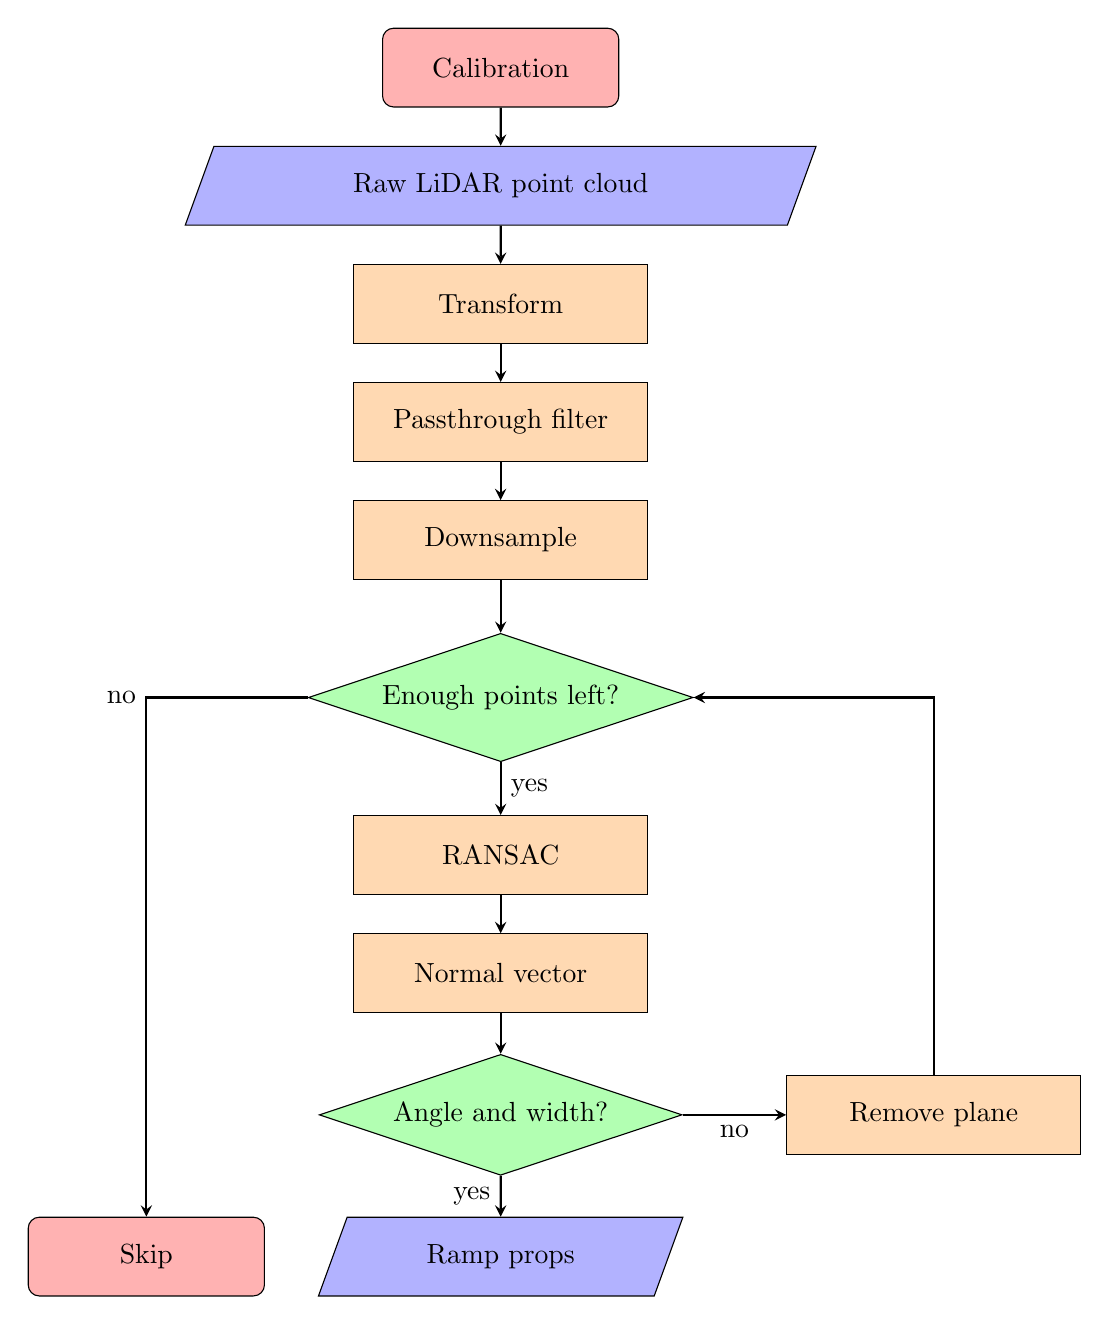
\begin{tikzpicture}[node distance=1.5cm]
    % \node (start) [startstop] {Start};
    % \node (raw) [io, below of=start] {Raw \acrshort{lidar} point cloud};
    \node (calibration) [startstop] {Calibration};
    \node (raw) [io, below of=calibration] {Raw LiDAR point cloud};
    \node (transform) [process, below of=raw] {Transform};
    \node (passthrough) [process, below of=transform] {Passthrough filter};
    \node (downsample) [process, below of=passthrough] {Downsample};
    \node (is_enough_points) [decision, below of=downsample, yshift=-0.5cm] {Enough points left?};
    \node (ransac) [process, below of=is_enough_points, yshift=-0.5cm] {RANSAC};
    \node (nv) [process, below of=ransac] {Normal vector};
    \node (is_ramp) [decision, below of=nv, yshift=-0.3cm] {Angle and width?};
    \node (reduce) [process, right of=is_ramp, xshift=4cm] {Remove plane};
    \node (rotmat) [io, below of=is_ramp, yshift=-0.3cm] {Ramp props};
    \node (skip) [startstop, left of=rotmat, xshift=-3cm] {Skip};
    % \node (end) [startstop, below of=rotmat] {Stop};


    % Connect the nodes
    % \draw [arrow] (start) -- (raw);
    \draw [arrow] (calibration) -- (raw);
    \draw [arrow] (raw) -- (transform);
    \draw [arrow] (transform) -- (passthrough);
    \draw [arrow] (passthrough) -- (downsample);
    \draw [arrow] (downsample) -- (is_enough_points);
    \draw [arrow] (is_enough_points) -- node[anchor=west] {yes} (ransac);
    \draw [arrow] (is_enough_points) -| node[anchor=east] {no} (skip);
    \draw [arrow] (ransac) -- (nv);
    \draw [arrow] (nv) -- (is_ramp);
    \draw [arrow] (is_ramp) -- node[anchor=east] {yes} (rotmat);
    \draw [arrow] (is_ramp) -- node[anchor=north] {no} (reduce);
    \draw [arrow] (reduce) |- (is_enough_points);
    % \draw [arrow] (rotmat) -- (end);
\end{tikzpicture}
\end{document}